\documentclass{beamer}

\usefonttheme{serif}

\usepackage{tikz}
\usebackgroundtemplate{
    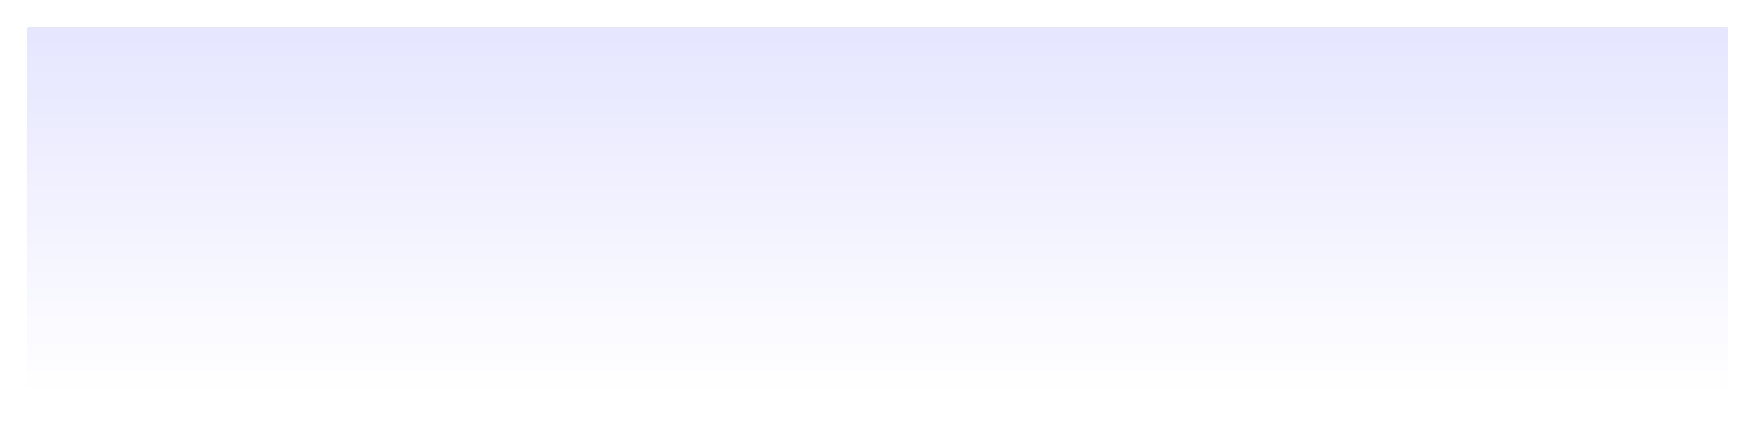
\begin{tikzpicture}
        \shade[top color=blue!10, bottom color=white] 
            (0,0) 
            rectangle 
            (\paperwidth, \paperheight/6);
    \end{tikzpicture}
}

% Clear Beamer Footer
\setbeamertemplate{footline}[frame number]{}
\setbeamertemplate{navigation symbols}{}
\setbeamertemplate{footline}{}

\setbeamertemplate{footline}
{
  \hbox{%
    \begin{beamercolorbox}[wd=1\paperwidth,ht=2.25ex,dp=1ex,center]{framenumber}%
        \usebeamerfont{framenumber}\insertframenumber{} / \inserttotalframenumber\hspace*{2ex}
    \end{beamercolorbox}}%
  \vskip10pt%
}

% Table of Contents at beginning of Section
\AtBeginSection[]
{
    \begin{frame}{Table of Contents}
        \tableofcontents[currentsection]
    \end{frame}
}


\usepackage{fontspec}

\usepackage{unicode-math}
\usepackage{mathtools}
\usepackage{amsmath}

\usepackage{csquotes}

\usepackage{hyperref}

\usepackage{float}

\usepackage{booktabs}

\usepackage{xcolor}


\setmainfont{Latin Modern Roman}
\setsansfont{Latin Modern Sans}
\setmonofont{Ubuntu Mono Ligaturized}
\setmathfont{Latin Modern Math}


\newcommand{\Subtitle}[1]
{
    {\small {#1}}       \\
    {\small \phantom{}}
}

\newcommand{\Keyword}[1]{\textcolor{blue}{{#1}}}

\DeclarePairedDelimiterX\set[1]\lbrace\rbrace{\def\given{\;\delimsize\vert\;}#1}

\DeclarePairedDelimiterX\VSBars[1]\lvert\rvert{#1}
\DeclarePairedDelimiterX\VDBars[1]{\lvert\lvert}{\rvert\rvert}{#1}

\newcommand{\Real}{\mathbb{R}}
\newcommand{\Rational}{\mathbb{Q}}
\newcommand{\Complex}{\mathbb{C}}
\newcommand{\Int}{\mathbb{Z}}
\newcommand{\PosInt}{\mathbb{Z}^{+}}
\newcommand{\NegInt}{\mathbb{Z}^{-}}
\newcommand{\NatNum}{\mathbb{N}}
\newcommand{\PosRat}{\mathbb{R}^{+}}
\newcommand{\NegRat}{\mathbb{R}^{-}}

\newcommand{\AlephZero}{\aleph_{0}}

\DeclareMathOperator{\Exists}{\exists}
\DeclareMathOperator{\Forall}{\forall}

\DeclareMathOperator{\Diff}{\backslash}

\newcommand{\AbsComplement}[1]{{#1}^{c}}

\newcommand{\True}{\mathrm{T}}
\newcommand{\False}{\mathrm{F}}

\newcommand{\Domain}[1]{\operatorname{domain}({#1})}
\newcommand{\Image}[1]{\operatorname{image}({#1})}

\newcommand{\Inverse}[1]{{#1}^{-1}}

\newcommand{\Permutate}[1]{\sigma({#1})}

\DeclareMathOperator{\Sign}{sgn}

\newcommand{\Mod}[1]{\ (\mathrm{mod}\ #1)}

\newcommand{\Encrypt}[3]{\mathrm{encrypt}_{#1, #2}(#3)}
\newcommand{\Decrypt}[3]{\mathrm{decrypt}_{#1, #2}(#3)}

\newcommand{\MatrixClass}[2]{\mathcal{M}(#1, #2)}

\newcommand{\rddots}{\reflectbox{$\ddots$}}

\newenvironment{detmatrix}[1]{%
  \left\vert\begin{array}{@{}*{#1}{c}@{}}
}{%
  \end{array}\right\vert
}

\newenvironment{augmatrix}[1]{%
  \left[\begin{array}{@{}*{#1}{c}|c@{}}
}{%
  \end{array}\right]
}

\newcommand{\Prob}[1]{\mathrm{P}(#1)}


\usetikzlibrary{shapes,arrows}


\newtheorem{remark}{Remark}



\title{
    \Subtitle{COMP0005 Algorithms}  \\
    {\huge\itshape Graphs}                  \\
}
\author{Jieyou Xu}
\date{\today}


\begin{document}
\frame{\titlepage}

\section{Introduction to Graphs}

\begin{frame}{Undirected Simple Graph}
    An \Keyword{undirected simple graph} $G$ is a two-tuple
    \begin{equation}
        G = (V, E)
    \end{equation}
    Where
    \begin{enumerate}
        \item $V$ is the set of \Keyword{vertices} (or \Keyword{nodes}, \Keyword{points})
        \item $E$ is the set of \Keyword{edges} (or \Keyword{links}) where each \Keyword{edge} connects two \Keyword{vertices}
        \begin{itemize}
            \item Not allowing \textit{self-loops}:
            \begin{equation}
                E \subseteq \set{(x, y) \mid (x, y) \in V^2 \land x \ne y}
            \end{equation}
            \item Allowing \textit{self-loops}:
            \begin{equation}
                E \subseteq \set{(x, y) \mid (x, y) \in V^2}
            \end{equation}
        \end{itemize}
    \end{enumerate}
\end{frame}

\begin{frame}
    No \textit{self-loops}
    \begin{figure}[H]
        \centering
        \begin{equation*}
            \psmatrix[colsep=2em, rowsep=1em, mnode=circle, linewidth=0.5pt]
                x & y
                \ncline{-}{1, 1}{1, 2}
            \endpsmatrix
        \end{equation*}
    \end{figure}
    
    Allowing \textit{self-loops}
    \begin{figure}[H]
        \centering
        \begin{equation*}
            \psmatrix[colsep=2em, rowsep=1em, mnode=circle, linewidth=0.5pt]
                x & y
                \ncline{-}{1, 1}{1, 2}
                \nccircle{-}{1, 2}{1em}
            \endpsmatrix
        \end{equation*}
    \end{figure}
\end{frame}

\begin{frame}{Directed Simple Graph}
    A \Keyword{directed simple graph} $G$ is a \textit{graph} in which \textit{edges} have orientation
    \begin{equation}
        G = (V, A)
    \end{equation}
    Where
    \begin{enumerate}
        \item $V$ is the set of \Keyword{vertices} (or \Keyword{nodes}, \Keyword{points})
        \item $A$ is the set of \Keyword{directed edges} where each \Keyword{edge} connects two vertices with a \Keyword{direction}
    \end{enumerate}
\end{frame}

\begin{frame}{Directed Edge}
    In a \Keyword{directed simple graph}, each \Keyword{edge} $(x, y)$ connects \textit{vertex} $x \to y$.
    \begin{figure}[H]
        \centering
        \begin{equation*}
            \psmatrix[colsep=2em, rowsep=1em, mnode=circle, linewidth=0.5pt]
                x & y
                \ncline{->}{1, 1}{1, 2}
            \endpsmatrix
        \end{equation*}
    \end{figure}
    For the \Keyword{directed edge} $(x, y)$ from $x \to y$
    \begin{itemize}
        \item $x$ is the \Keyword{tail} of the edge
        \item $y$ is the \Keyword{head} of the edge
    \end{itemize}
    
    The \Keyword{edge} $(y, x)$ is the \Keyword{inverted edge} of $(x, y)$
    \begin{figure}[H]
        \centering
        \begin{equation*}
            \psmatrix[colsep=2em, rowsep=1em, mnode=circle, linewidth=0.5pt]
                x & y
                \ncline{->}{1, 2}{1, 1}
            \endpsmatrix
        \end{equation*}
    \end{figure}
\end{frame}

\begin{frame}{Directed Edge}
    It is also possible for a \textit{loop} (or \textit{cycle}) to form between nodes
    \begin{figure}[H]
        \centering
        \begin{equation*}
            \psmatrix[colsep=2em, rowsep=1em, mnode=circle, linewidth=0.5pt]
                x & y
                \ncarc[arcangle=45]{->}{1, 1}{1, 2}
                \ncarc[arcangle=45]{->}{1, 2}{1, 1}
            \endpsmatrix
        \end{equation*}
    \end{figure}
\end{frame}

\end{document}
